\documentclass[tikz,border=10pt]{standalone}
\usepackage{amsmath}
\begin{document}
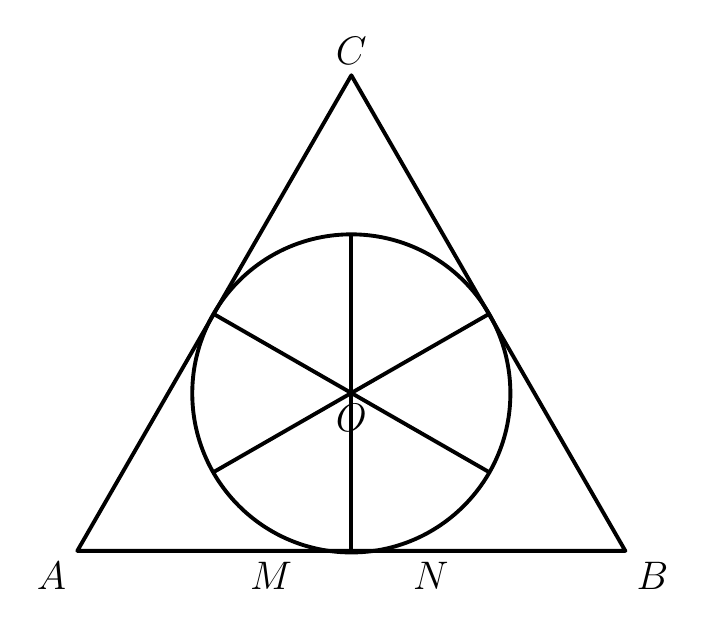
\begin{tikzpicture}[line width=1.4pt, line join=round]
  % Coordinates: s = 0.017021 cm/px, origin at ink-bbox centre (271.7, 242.5)
  \coordinate (C) at (0.00,3.02);
  \coordinate (A) at (-3.48,-3.02);
  \coordinate (B) at (3.48,-3.02);
  \coordinate (O) at (0.00,-1.02);
  \coordinate (T) at (0.00,-3.02);
  % Top of incircle: O + (0, r), r = 2.02
  \coordinate (Top) at (0.00,1.00);
  % Chords through O at +30 and -30 degrees, ending on the incircle
  \coordinate (P1) at (-1.75,-2.02);
  \coordinate (P2) at (1.75,-0.01);
  \coordinate (Q1) at (-1.75,-0.01);
  \coordinate (Q2) at (1.75,-2.02);
  \coordinate (M) at (-1.02,-3.02);
  \coordinate (N) at (1.01,-3.02);

  % Triangle
  \draw (C) -- (A) -- (B) -- cycle;

  % Incircle, centre O, radius 2.02
  \draw (O) circle[radius=2.02];

  % Vertical segment: top on incircle top, bottom at tangent point T on AB
  \draw (Top) -- (T);
  \draw (P1) -- (P2);
  \draw (Q1) -- (Q2);

  % Labels
  \node[above, font=\fontsize{13.5}{16.2}\selectfont] at (C) {$C$};
  \node[below left, font=\fontsize{13.5}{16.2}\selectfont] at (A) {$A$};
  \node[below right, font=\fontsize{13.5}{16.2}\selectfont] at (B) {$B$};
  % O label directly below the centre
  \node[anchor=north, font=\fontsize{13.5}{16.2}\selectfont] at (O) {$O$};
  \node[below, font=\fontsize{13.5}{16.2}\selectfont] at (M) {$M$};
  \node[below, font=\fontsize{13.5}{16.2}\selectfont] at (N) {$N$};
\end{tikzpicture}
\end{document}